\begin{figure}[ht]
    \centering
    \vspace{-3mm}
    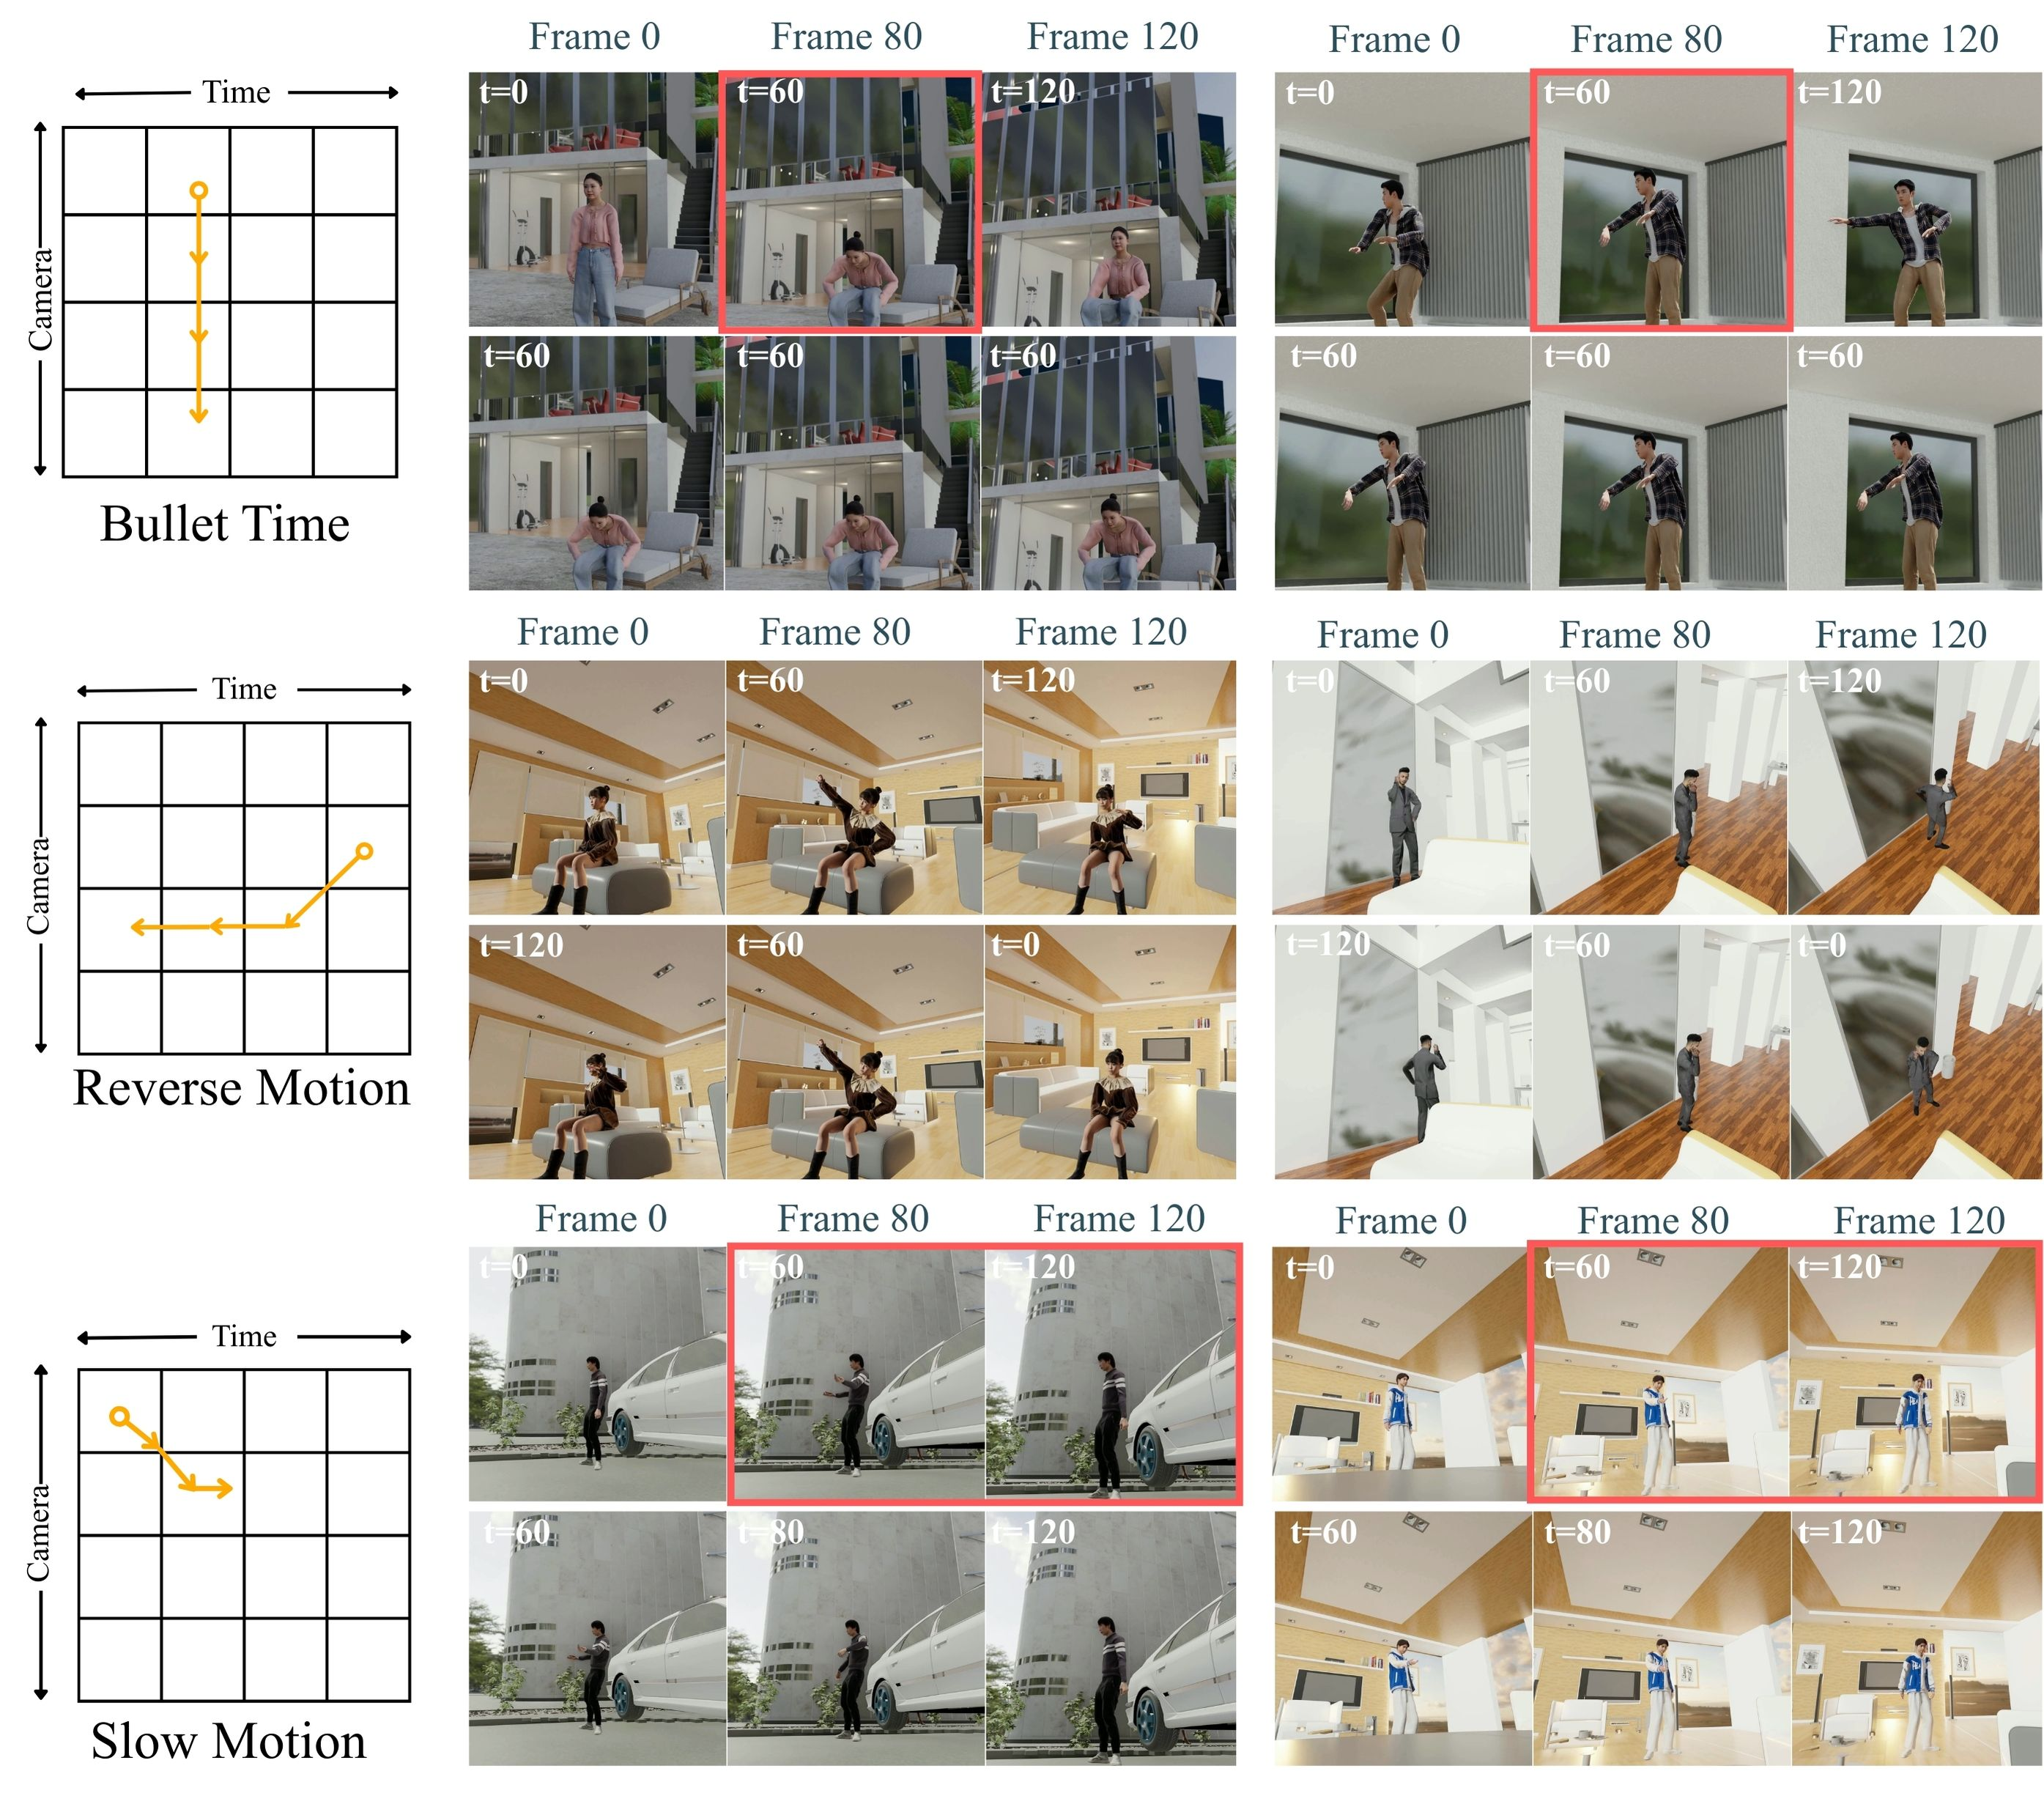
\includegraphics[width=\linewidth]{figures/src_files/sampling_example.jpg}
    
    \caption{
    \textbf{Sampling from \nameDataset.}
By sampling from the \nameDataset dataset, we can extract frames corresponding to arbitrary combinations of camera viewpoints and temporal positions, forming source-target pairs with rich camera and temporal control signals.
    }
    \label{fig:sampling}
\end{figure}
